\documentclass[onecolumn]{article}
%\usepackage{url}
%\usepackage{algorithmic}
\usepackage[a4paper]{geometry}
\usepackage{datetime}
\usepackage[margin=2em, font=small,labelfont=it]{caption}
\usepackage{graphicx}
\usepackage{mathpazo} % use palatino
\usepackage[scaled]{helvet} % helvetica
\usepackage{microtype}
\usepackage{amsmath}
\usepackage{subfigure}
\usepackage{float}
% Letterspacing macros
\newcommand{\spacecaps}[1]{\textls[200]{\MakeUppercase{#1}}}
\newcommand{\spacesc}[1]{\textls[50]{\textsc{\MakeLowercase{#1}}}}

\title{\spacecaps{FACE DETECTION PROJECT}\\ \normalsize \spacesc{ DATA MINING} }

\author{Emre Taşkın\\emretaskin2@mu.edu.tr}

\begin{document}
\maketitle

\begin{abstract}
In this project, I tried to make a face recognition program, which can make predictions about a face image's reality. The program is going to output two results which are fake and real.
\end{abstract}


\section{Introduction}
Face detection is a fundamental problem in many computer vision applications, so that I wanted to work with an image dataset. I collected my data from kaggle.

\section{Assignments}
I used Keras, Tensorflow, Matplotlib, Numpy and Juptyer Notebook with Pyhton.
\subsection{Assignment 2.1}

I used kera's ImageDataGenerator to not only label the data, also to slightly augment the data with shifts, rotations, zooms, and mirroring. Mirroring helped to ensure that the data was not biased to a particular handedness.

\begin{figure}[H]
\centering
    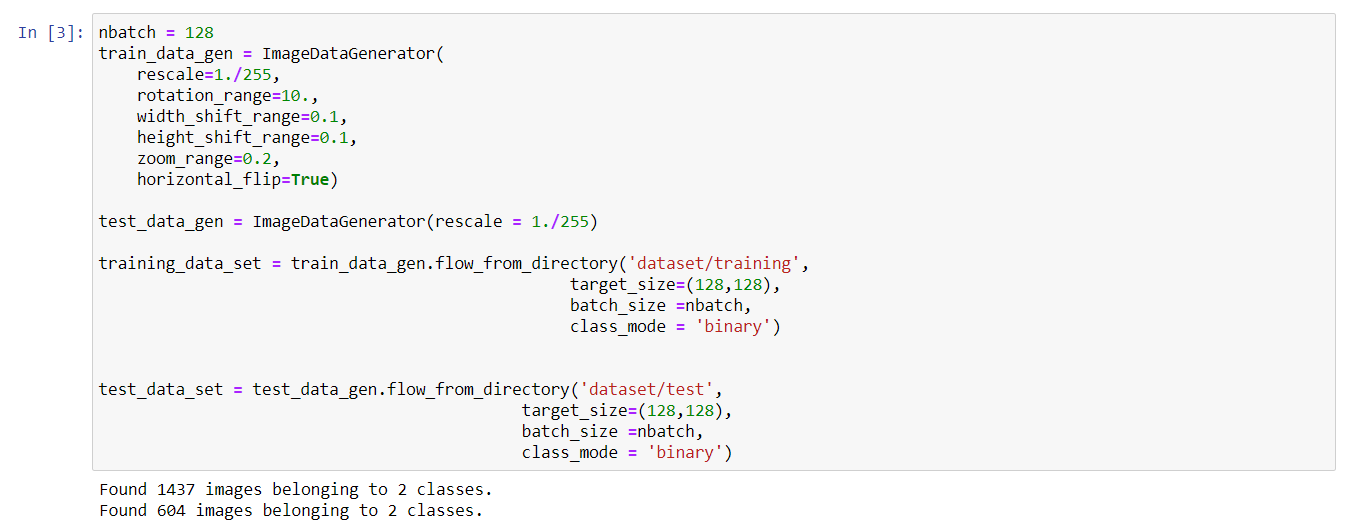
\includegraphics[width=1\linewidth]{assg1.png}
\caption{}
\end{figure}

\begin{figure}[H]
\centering
    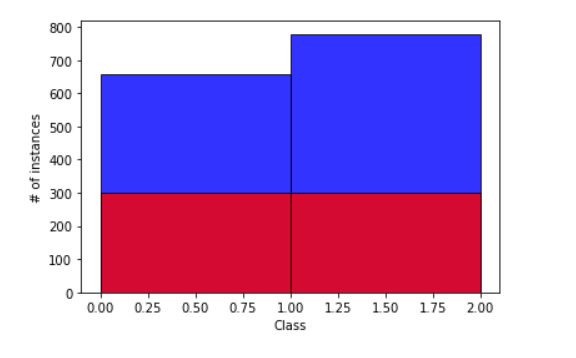
\includegraphics[width=1\linewidth]{graph.png}
\caption{ Here is the graph class and instance graph of my data.}
\end{figure}


\subsection{Assignment 2.2}

I defined a Convolutional Neural Network model to train and use in my application.


\begin{figure}[H]
\centering
    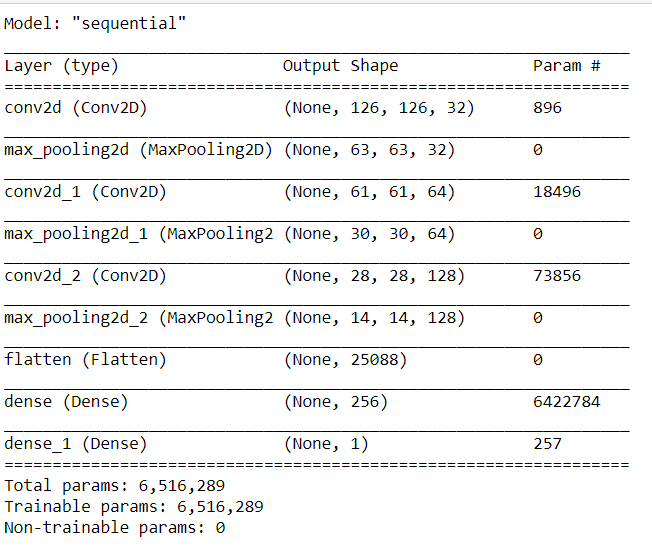
\includegraphics[width=1\linewidth]{assg2.png}
\caption{then I compiled the model}
\end{figure}

\subsection{Assignment 2.3}
I trained my model by using some helper functions of keras.

\begin{figure}[H]
\centering
    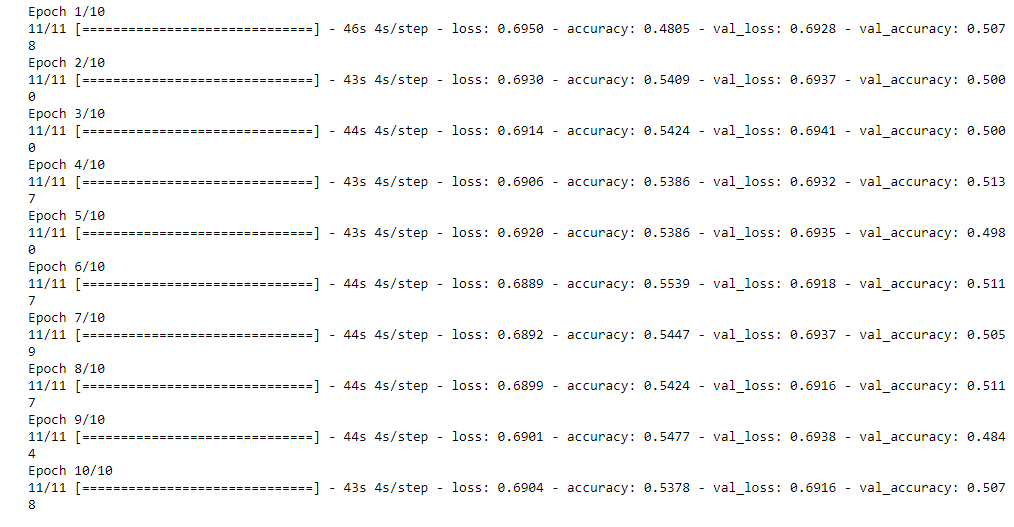
\includegraphics[width=1\linewidth]{assg3.png}
\caption{}
\end{figure}


\begin{figure}[H]
\centering
    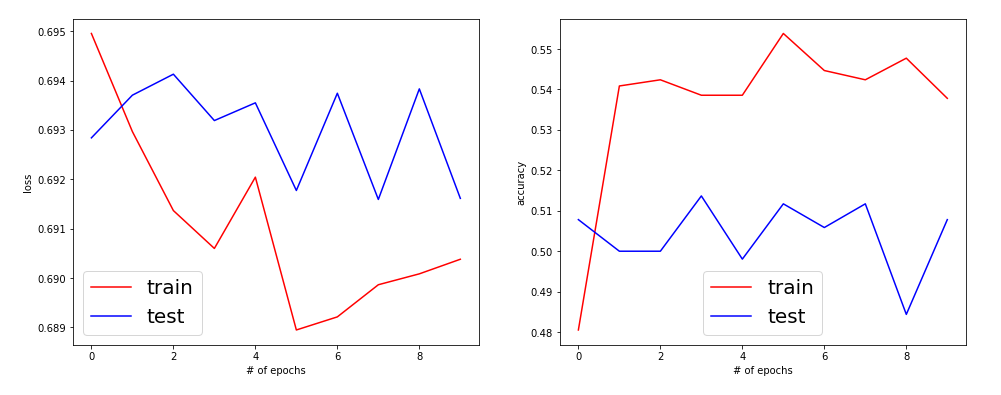
\includegraphics[width=1\linewidth]{assg33.png}
\caption{loss and accuracy graphs}
\end{figure}


\section{Results}

After I trained the model , I used some images to see my project working well or not.

\begin{figure}[H]
\centering
    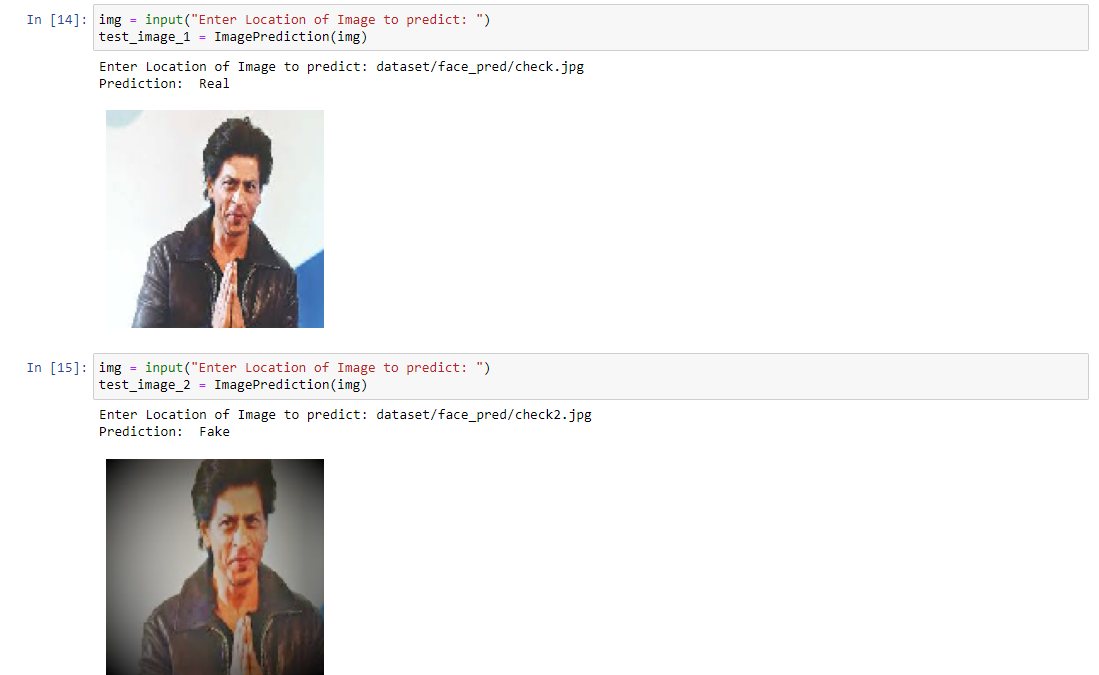
\includegraphics[width=1\linewidth]{result1.png}
\caption{}
\end{figure}

\begin{figure}[H]
\centering
    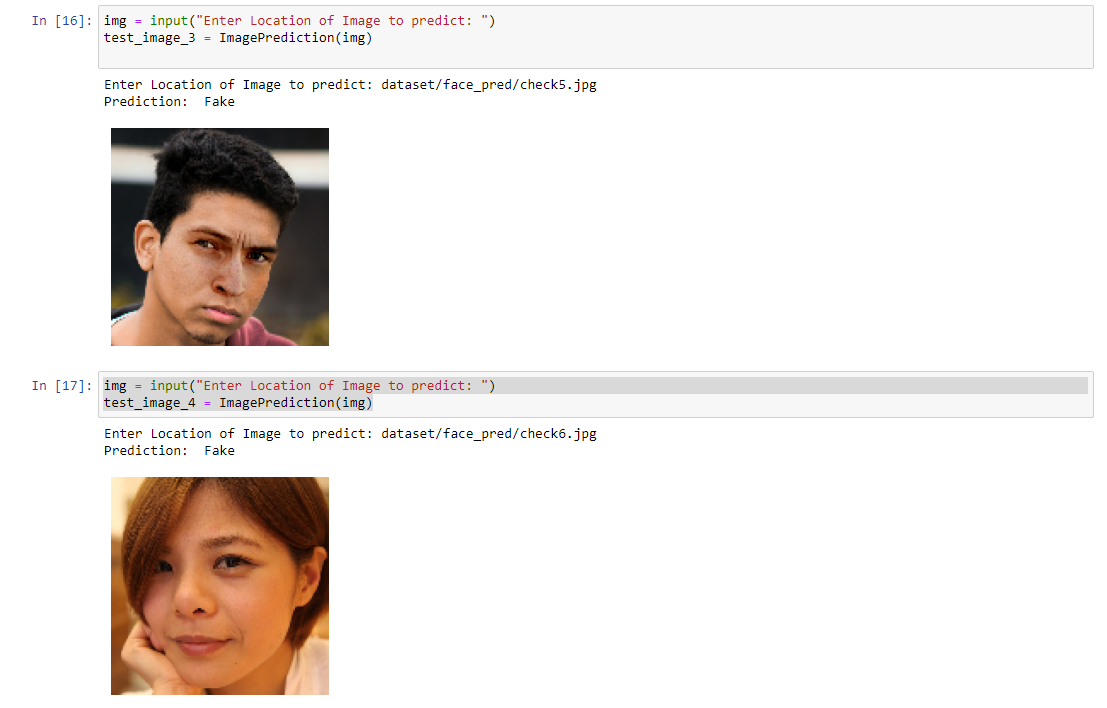
\includegraphics[width=1\linewidth]{res2.png}
\caption{}
\end{figure}


\section{Conclusion}
In this project I learned using keras and tensorflow libraries in python. Working with images was a good experience for me. Some of images is predicted correctly althrough model is not trained well. Incereasing epoc will probably make this model perfectly trained but that will take long time for training and this training will need high computer performance.


\nocite{*}
\bibliographystyle{plain}
\bibliography{references}
\end{document}

